\documentclass[12pt]{beamer}
\usepackage[utf8]{inputenc}
\usepackage{amsmath}
\usepackage{amsfonts}
\usepackage{amssymb}
\usepackage{graphicx}
\usepackage{hyperref}
\usepackage{url}
\usepackage{listings}

\lstdefinelanguage{scala}{
  morekeywords={abstract,case,catch,class,def,%
    do,else,extends,false,final,finally,%
    for,if,implicit,import,match,mixin,%
    new,null,object,override,package,%
    private,protected,requires,return,sealed,%
    super,this,throw,trait,true,try,%
    type,val,var,while,with,yield},
  otherkeywords={=>,<-,<\%,<:,>:,\#,@},
  sensitive=true,
  morecomment=[l]{//},
  morecomment=[n]{/*}{*/},
  morestring=[b]",
  morestring=[b]',
  morestring=[b]"""
}

\usepackage{color}
\definecolor{dkgreen}{rgb}{0,0.6,0}
\definecolor{gray}{rgb}{0.5,0.5,0.5}
\definecolor{mauve}{rgb}{0.58,0,0.82}
\lstset{frame=tb,
  language=scala,
  aboveskip=3mm,
  belowskip=3mm,
  showstringspaces=false,
  columns=flexible,
  basicstyle={\small\ttfamily},
  numbers=none,
  numberstyle=\tiny\color{gray},
  keywordstyle=\color{blue},
  commentstyle=\color{dkgreen},
  stringstyle=\color{mauve},
  frame=single,
  breaklines=true,
  breakatwhitespace=true
  tabsize=3
}

\usetheme{amsterdam}
\setbeamertemplate{navigation symbols}{}

\setbeamertemplate{footline}
{
    \begin{beamercolorbox}[wd=1\paperwidth,ht=2.25ex,dp=1ex,right]{date in head/foot}
    \usebeamerfont{date in head/foot}
    \insertshortauthor{}\hspace*{2em}
    \insertframenumber{} / \inserttotalframenumber\hspace*{2ex}
    \end{beamercolorbox}
}


\newcommand{\vcenteredinclude}[1]{\begingroup
\setbox0=\hbox{\includegraphics[height = 0.7cm]{#1}}%
\parbox{\wd0}{\box0}\endgroup}


\title[Pong Designer]{Pong Designer}
\subtitle{Another point of view}
\author[L. Mégard]{Lomig Mégard}
\institute[EPFL]{
  LARA\\
  Ecole polytechnique fédérale de Lausanne\\[1ex]
  \texttt{lomig.megard@epfl.ch}
}
\date[June 2013]{June 13, 2013}

\begin{document}

\begin{frame}[plain]
\titlepage
\end{frame}

\begin{frame}{Pong Designer}
The user defines both the state and the \textbf{behaviour} using the programming by demonstration paradigm:\\[1em]
\begin{itemize}
\item The user creates a state where the pre-condition occurs
\item Go back in time to select it
\item Modify the state to show the post-conditions
\item The game engine infers an appropriate rule
\end{itemize}
\end{frame}

\begin{frame}{Issues of the old implementation}
\begin{itemize}
\item Proof of concept
\item Physics engine hard to maintain and debug
\item Tunnelling effect
\item Poor modularity
\end{itemize}
\end{frame}

\begin{frame}{Goals of the new implementation}
\begin{itemize}
\item Dedicated physics engine
\item New ASTs for rules.
\item Support to group of objects
\item Maintainability and modularity
\end{itemize}
\end{frame}

\begin{frame}[t]{Overview}
\begin{itemize}
\item Architecture
\item Statements and expressions
\item Type system
\item Rules
\item Categories
\item Time management
\item Physics engine
\item Game objects
\item One time step
\item Future work
\item Conclusion
\end{itemize}
\end{frame}

\begin{frame}{Architecture - 1}
\centering
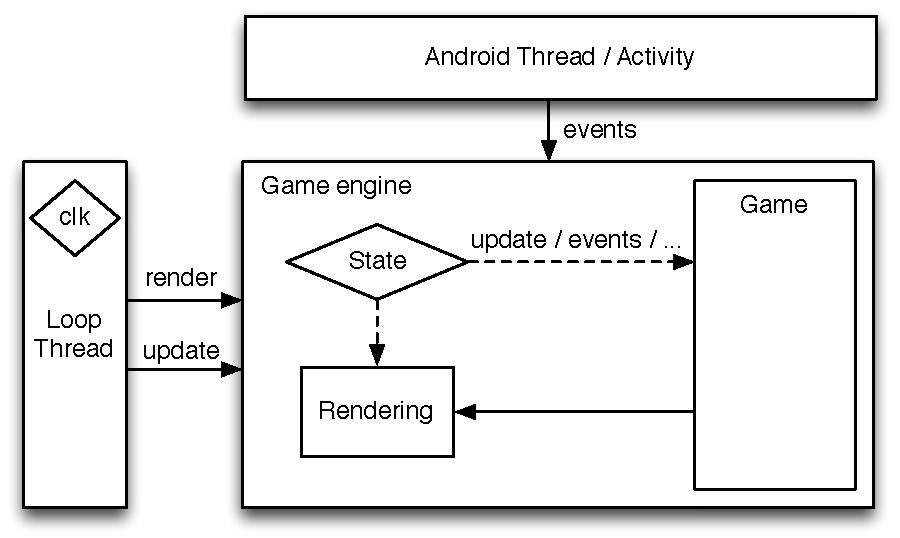
\includegraphics[scale=0.7]{images/architecture-1}
\end{frame}

\begin{frame}{Architecture - 2}
\centering
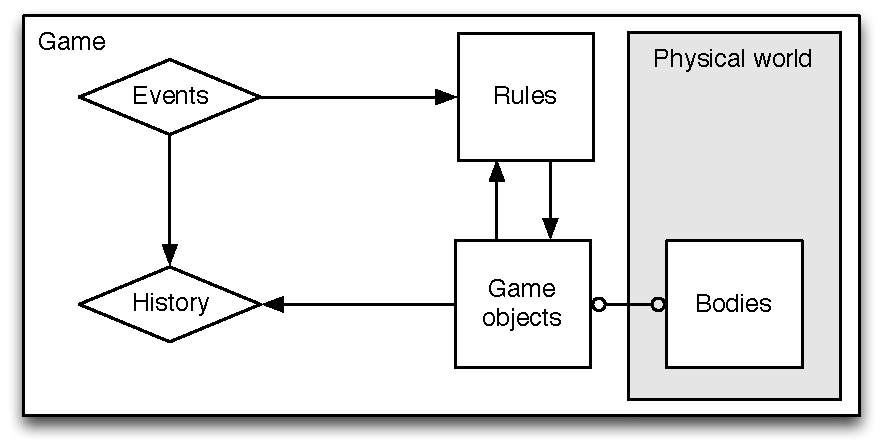
\includegraphics[scale=0.7]{images/architecture-2}
\end{frame}

\begin{frame}[fragile]{Statements and expressions - 1}
\begin{itemize}
\item Permit to modify the rules, to reason about them
\item Use of AST: convenient to manipulate
\item Runtime typechecker and interpreter
\item Statement with side-effects, without type
\item Expressions without side-effects, with type
\end{itemize}
\end{frame}

\begin{frame}[fragile]{Statements and expressions - 2}
\begin{lstlisting}
circle("x") := circle("x") + 1
\end{lstlisting}
\begin{center}
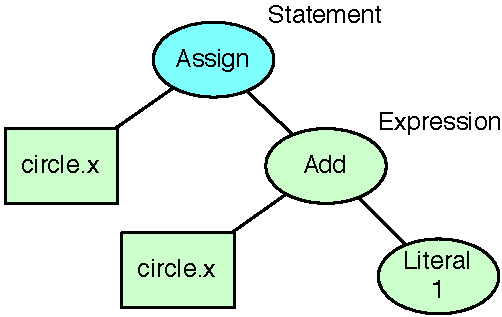
\includegraphics[scale=0.9]{images/AST_example}
\end{center}
\end{frame}


\begin{frame}[fragile]{Type system - 1}
Each object property has two linked types:
\begin{itemize}
\item the expression type (use type classes)
\item the value type (use Scala types)
\end{itemize}

\vspace*{5mm}

\begin{lstlisting}
abstract class Property[T : PongType](...) {
  def get: T
  def tpe = implicitly[PongType[T]]
  ...
}
\end{lstlisting}

\end{frame}


\begin{frame}[fragile]{Type system - 2}
Benefit from the two types:
\begin{itemize}
\item the user can build expression with properties
\item the game engine is typesafe
\end{itemize}

\vspace*{5mm}

\begin{lstlisting}
def evaluate[T : PongType](e: Expr): T = {
  typeCheck(e, implicitly[PongType[T]].getPongType)
  eval(e)(EventHistory).as[T]
}
\end{lstlisting}

\end{frame}


\begin{frame}[fragile]{Rules}
Permit to change the game state.
\begin{itemize}
\item One boolean expression for condition
\item One statement for body
\item Several triggers: \texttt{Whenever}, \texttt{On} and \texttt{Once}
\end{itemize}

\vspace*{5mm}

\begin{lstlisting}
whenever(Collision(ball, brick)) { Seq(
  brick("visible") := false, 
  score("value") += 1
)}
\end{lstlisting}
\end{frame}

\begin{frame}[fragile]{Categories}

\begin{itemize}
\item Unified behaviour for a group of objects
\item Each object has one category
\item Rules don't accept categories, use \texttt{foreach} to iterate
\end{itemize}

\begin{lstlisting}
val bricks = new Category("Bricks")
rectangle("b1", x = 1, y = 0).withCategory(bricks)
rectangle("b2", x = 3, y = 0).withCategory(bricks)

val rule = foreach(bricks) { brick =>
  whenever(Collision(ball, brick)) { Seq(
    brick("visible") := false,
    score("value") += 1
  )}
}
\end{lstlisting}
\end{frame}

\begin{frame}{Time management}
Go back in time to create new rules.
\begin{itemize}
\item Store game state at each time step
\item Use a \texttt{RingBuffer} to handle bounded history
\end{itemize}
\end{frame}

\begin{frame}{Physics engine}
\begin{itemize}
\item Dedicated physical world using JBox2D
\item Only basic features are currently used
\item Each JBox2D body is wrapped by a \texttt{GameObject}
\item A \texttt{GameObject} handles its history and does the bridge with the type system
\end{itemize}
\end{frame}

\begin{frame}{Game objects}
A \texttt{GameObject} handles its history and does the bridge with the type system
 
\begin{center}
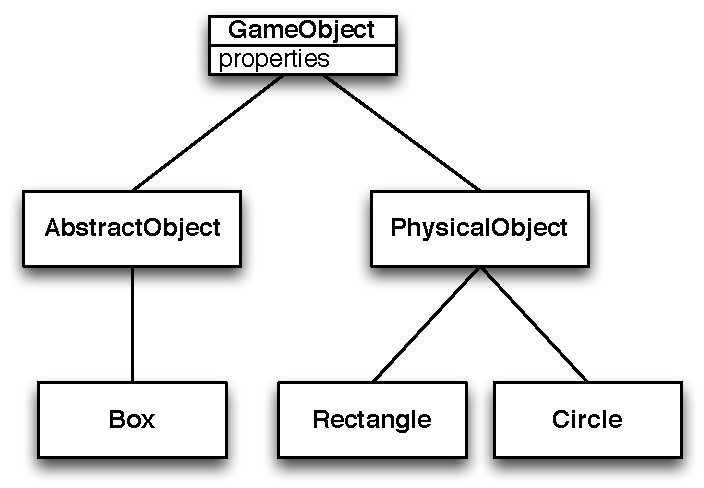
\includegraphics[scale=0.65]{images/objects}
\end{center}

\end{frame}

\begin{frame}{One time step}

Fixed discrete time step. One game update is:
\vspace*{2mm}
\begin{enumerate}
\item Evaluate the rules;
\item New values are flushed to the physics engine;
\item Update the physical world using JBox2D;
\item Load new values from the physics engine;
\item Save the current state in the history.
\end{enumerate}

\end{frame}

\begin{frame}{Future work}
This project produced multiple building bricks. The next step is to use them:
\begin{itemize}
\item Integrate the inferencer on top of these bricks
\item Port the old UI to the new implementation
\end{itemize}
\end{frame}


\begin{frame}{Conclusion}
\begin{itemize}
\item Good design takes time
\item JBox2D is fast but not quick to learn
\item Scala runs smoothly on Android 
\end{itemize}
\end{frame}

\end{document}